\documentclass[9pt,english]{beamer}
    % language: "english" (default), "german", "ngerman"
\usetheme{weierstrass}
\usepackage[utf8]{inputenc}
    % input encoding, maybe you want "latin1" or "ansinew"

\title[Short Title]{Long long long Title}
\author{Max Mustermann, Moritz Mustermann, Maria Musterfrau}
\date{WIAS, \today}
% change logos on the right side of title page
%\logos{\mbox{}\hfill
\includegraphics[height=2cm]{tiger}}

\begin{document}
% Create title page from data entered above.
\maketitle   % or \frame[plain]{\maketitle}

\begin{frame}
  \frametitle{About WIAS}
  \begin{columns}
    \begin{column}{.45\linewidth}
      \Large WIAS

      \begin{itemize}
        \item conducts project-oriented research in applied mathematics
        \item runs research projects in main application areas covering complex problems from economics, science and technology
        \item is named after the Berlin mathematician Karl Weierstrass
      \end{itemize}
    \end{column}
    \begin{column}{.45\linewidth}
      \centering
      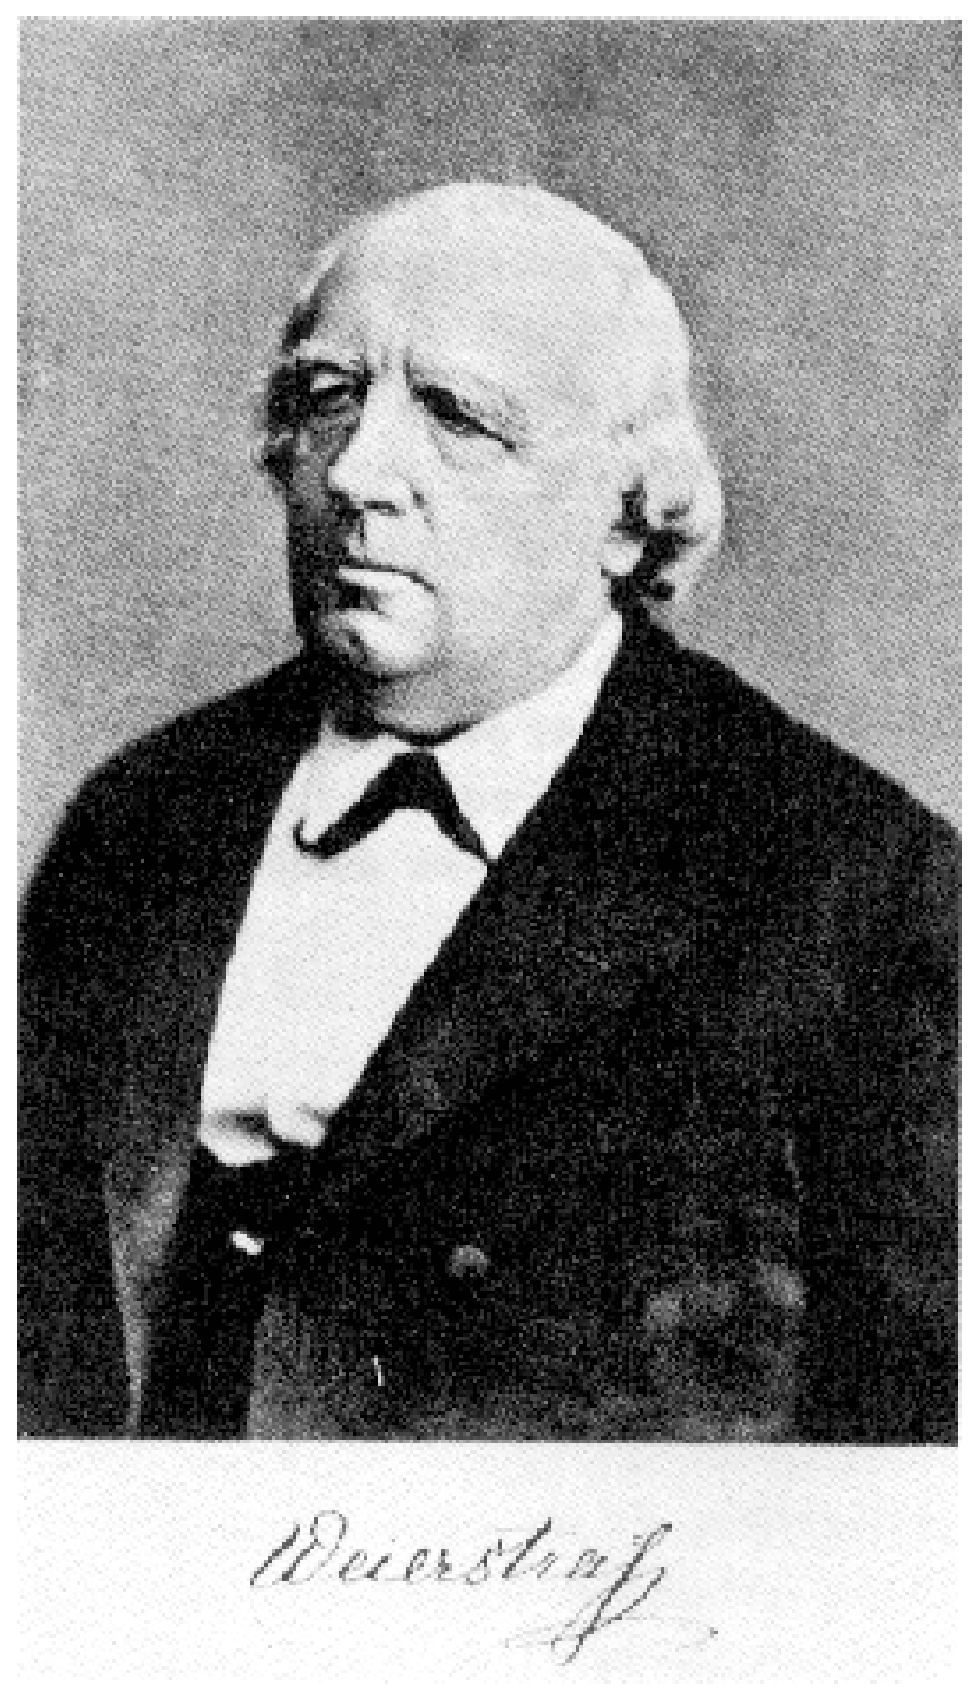
\includegraphics[height=\textheight]{kweierstrass}
    \end{column}
  \end{columns}
\end{frame}

% Print table of contents at begin of talk.
\tocatbegin
% Print table of contents at begin of each section.
\tocatsection
\section{One Section}
\subsection{\ldots\ with Subsection}
\begin{frame}{Blindtext}
Hello, here is some text without a meaning. This text should show, how a
printed text will look like at this place. If you read this text, you will
get no information. Really? Is there no information? Is there a difference
between this text and some nonsense like »Huardest gefburn«? Kjift – Never
mind! A blind text like this gives you information about the selected font,
how the letters are written and the impression of the look. This text
should contain all letters of the alphabet and it should be written in of
the original language. There is no need for a special contents, but the
length of words should match to the language.
\end{frame}
\begin{frame}{Itemize}
\begin{itemize}
  \item First item in a list
  \item Second item in a list
  \item Third item in a list
  \item Fourth item in a list
  \item Fivth item in a list
\end{itemize}
\end{frame}
\section{Another Section}
\subsection{\ldots\ and Subsection}
\begin{frame}{Enumerate}
\begin{enumerate}
  \item First item in a list
  \item Second item in a list
  \item Third item in a list
  \item Fourth item in a list
  \item Fivth item in a list
\end{enumerate}
\end{frame}
\begin{frame}{Blocks}
  \begin{block}{Normal Block}
    Some content.
  \end{block}
  \begin{exampleblock}{Example Block}
    Some content.
  \end{exampleblock}
  \begin{alertblock}{Alert Block}
    Some content.
  \end{alertblock}
  \begin{theorem}
    $a^2+b^2=c^2$
  \end{theorem}
  \begin{proof}
    Trivial. \\
    Exercise.
  \end{proof}
\end{frame}
\end{document}
